\section{Application and Models}
\subsection{Application}
\label{section:application}
In this paper, we focus on a particular type of regression task on multi-dimensional time-series data: air pollutant forecast of \textbf{target pollutants} at \textbf{target locations}.
We collaborate with a group of domain researchers who use RNNs to conduct air pollutant forecasting.
Specifically, they choose 16 air quality monitoring stations in Hong Kong with the stations' locations as the \textbf{target locations} and select $PM_{2.5}$, $PM_{10}$, $NO_{2}$, $SO_{2}$, and $O_3$ as the \textbf{target pollutants}.
Though the RNNs can provide high accuracy, the researchers are more interested in understanding why the models make certain predictions so that they can decide whether to trust the models for decision making based on their domain knowledge.
% \zw{needs more details here. analytical goals come too late. move here?}
We thus develop MultiRNNExplorer to help the domain researchers explain the RNNs' behavior on their temporal multi-dimensional air pollutant dataset.


% According to the requirement, for each model, on of the 16 air quality monitoring stations at Hong Kong as are chosen as\textbf{ target station}. 
% \yh{We may only describe our task and end users in Sec. 3.1 and remove other materials.}
% Our targeted problem is understanding RNN behaviour in air pollutant forecast. 
% The air pollutant has raised more and more attention of researchers. 
% As one of the most studied problems, traditional techniques such as CMAQ(Community Multi-scale Air Quality)~\cite{byun1999science} and ADMS-Urban~\cite{stocker2012adms} have been developed for long time air quality forecasting.
% However, the accuracy of these techniques relies on an updated pollutant source list which is very difficult to produce and update ~\cite{xi2015comprehensive}.
% Machine learning techniques are applied in this task~\cite{zhou2017prediction, reddy2018deep, ong2016dynamically} for the precise short-term prediction since it can leverage the real-time observation data. 

% \QM{Here we need to discuss the end user? This paragraph should be modified.}

% With the fast development of machine learning tools such as Tensorflow, Keras, Pytorch and Caffe, it becomes easier and easier for the environment researchers with no deep knowledge of machine learning to design and train models for the forecasting tasks. 
% Strobelt et al.\cite{strobelt2018lstmvis} has summarized three users roles: architects, trainers and end users. Our target users is between the trainer and end user. They utilize RNNs as tool and have domain knowledge about the atmosphere and air quality. They want to explore what the model learn and exam if the model capture reasonable factors to the forecasting.   



\subsection{Data Description}
\label{section:datadescription}

The dataset includes hourly observations of the air pollutant and meteorology data from different air quality monitoring stations in China from Jan. 01 2015 to Dec. 31 2018.
The features are listed in Table ~\ref{table:feature_list}.

\begin{table}[h!]
\centering
\caption{There are two types of features taken as input: air pollution and meteorology. }
\begin{tabular}{|p{2cm}|p{5.2cm}|} 
\hline
 Category & Feature type \\ [0.5ex] 
\hline
    Air pollutant&$PM_{2.5}$, $PM_{10}$, $NO_{2}$, $NO_{x}$, $SO_{2}$, $CO$, $O_3$\\[0.4ex] 
\hline
    Meteorology&\textit{Wind Speed(Wind), Wind Direction(WD), Dew Point(DP), Relative Humidity(RH), Temperature(Temp), Sea Level Pressure(SLP), Station Pressure(SP), Cloud Cover(CC)}\\
\hline
\end{tabular}
\label{table:feature_list}
\end{table}

% Since the monitoring stations which are too far away from the target locations have very few influence to the target location, the model only takes the observations from nearby stations as the input.
% Furthermore, even the spatial distance of the neighbor stations are limited, if all observations are fed into the model directly still cause trouble in the training and prediction with limit training data because the features collected from the stations may be redundant. 
Similar to other work on air pollutant forecasts~\cite{zheng2015forecasting}, when forecasting the air pollutants at a target location, we divide the regions around the target location into different spatial partitions and aggregate the data observed by all the stations within each group in order to generate features.
% Inspired by~\cite{zheng2015forecasting}, a similar spatial partition method are applied to aggregate the observation features(~\QM{as Fig.\ref{fig:teaser} B}). 
% \yh{Above sentences may be confusing...need discuss}
Specifically, as shown in Fig.~\ref{fig:teaser}B, we divide the nearby regions into five non-overlapping rings centered at the targeted location with radii of 10km, 30km, 100km, 200km, and 300km.
Each ring is further divided into 8 sectors with the same angle such that the whole area around the target location is partitioned into 40 sub-regions. 
For each sub-region, we use the air pollutant and meteorology data observed by the monitoring stations located in the corresponding sub-region as the features.
If there are multiple monitoring stations in a sub-region, we aggregate their data and use mean values as the features.
% The same features from the monitoring station located into a same region within a same time range(e.g. 1 hour) will be averaged by mean value of this region. 
In this way, each feature can be identified as a triplet $(distance, direction, feature\_type)$; for example, $(10km, E, NO_{2})$ indicates $NO_{2}$ concentration observed at \textit{10km} away \textit{East} of the target location. 
For each time step, we use a vector to represent all the features where each dimension indicates a feature triplet.
In this way, the data within a time peroid can be represented as a multi-dimensional sequence. 
% \QM{For each timestamp, we format all of the aggregated features at same timestamp as high-dimensional data and the data within a time range as a high-dimensional sequence.}

\subsection{Models Description}
\label{section:model_description}
RNNs take a sequence as input with fixed length $T$: $\{x_0, x_1,... x_{T-1}\}$ and predict the value at timestamps equal to or greater than $T$, where $x_{t} \in \mathbb R^{m}$. 
% To train and test the model, we use a sliding-window method with the window size between 6 and 48 to gradually scan all time-series data.
% \UC{So in the testing process, the input data $x$ will be read $T$ times and generate $T$ outputs from the hidden units.}
% \yh{To me, above 2 sentences describe how we generate sequences from data and can be removed / or moved to the data description sec.. I feel it is not direcctly relevant to model description.}
% and $x_{t}^k \in x_{t}$ is the value of $k^{th}$ at time-stamp $t$. Each dimension of $x$ are scaled in the range of [0, 1]. 
A hidden state $h_t$ is updated according to the input of timestamp $t$ and previous hidden state $h_{t-1}$.
\QM{In vanilla RNNs, the hidden states are updated by:} 
\begin{equation} 
h_t = \sigma(Wh_{t-1} + Vx_t)
\end{equation}

Where $W$ and $V$ are weight matrices and $\sigma$ is the $tanh$ function which constrains the output of the hidden states to $(-1, 1)$. We consider three types of architectures shown as Fig.~\ref{fig:model_type}. 
\textbf{RNN}: the final timestamp hidden state is directly connected to the output layer (Fig.~\ref{fig:model_type}A). \textbf{RNN-Dense}: there are several dense layers between the final timestamp and output layer (Fig.~\ref{fig:model_type}B). 
% In model of Fig.\ref{fig:model_type}A, the final time-stamp hidden state is directly connected to the output layer. For the model of Fig.\ref{fig:model_type}B, there are several dense layers between the final time-stamp and output layer. The model of Fig.\ref{fig:model_type}C has time-distributed dense layer between the RNN layer and output layer. In theory, the time-distributed layer can better capture the temporal dynamics\cite{teijeiro2017arrhythmia}.
In addition to vanilla RNNs, we also consider two variants: GRU and LSTM, which mitigate the gradient vanishing issue and enable the models to memorize long-term information by adding the ``gating'' mechanism.


\begin{figure}[t]
	\centering
    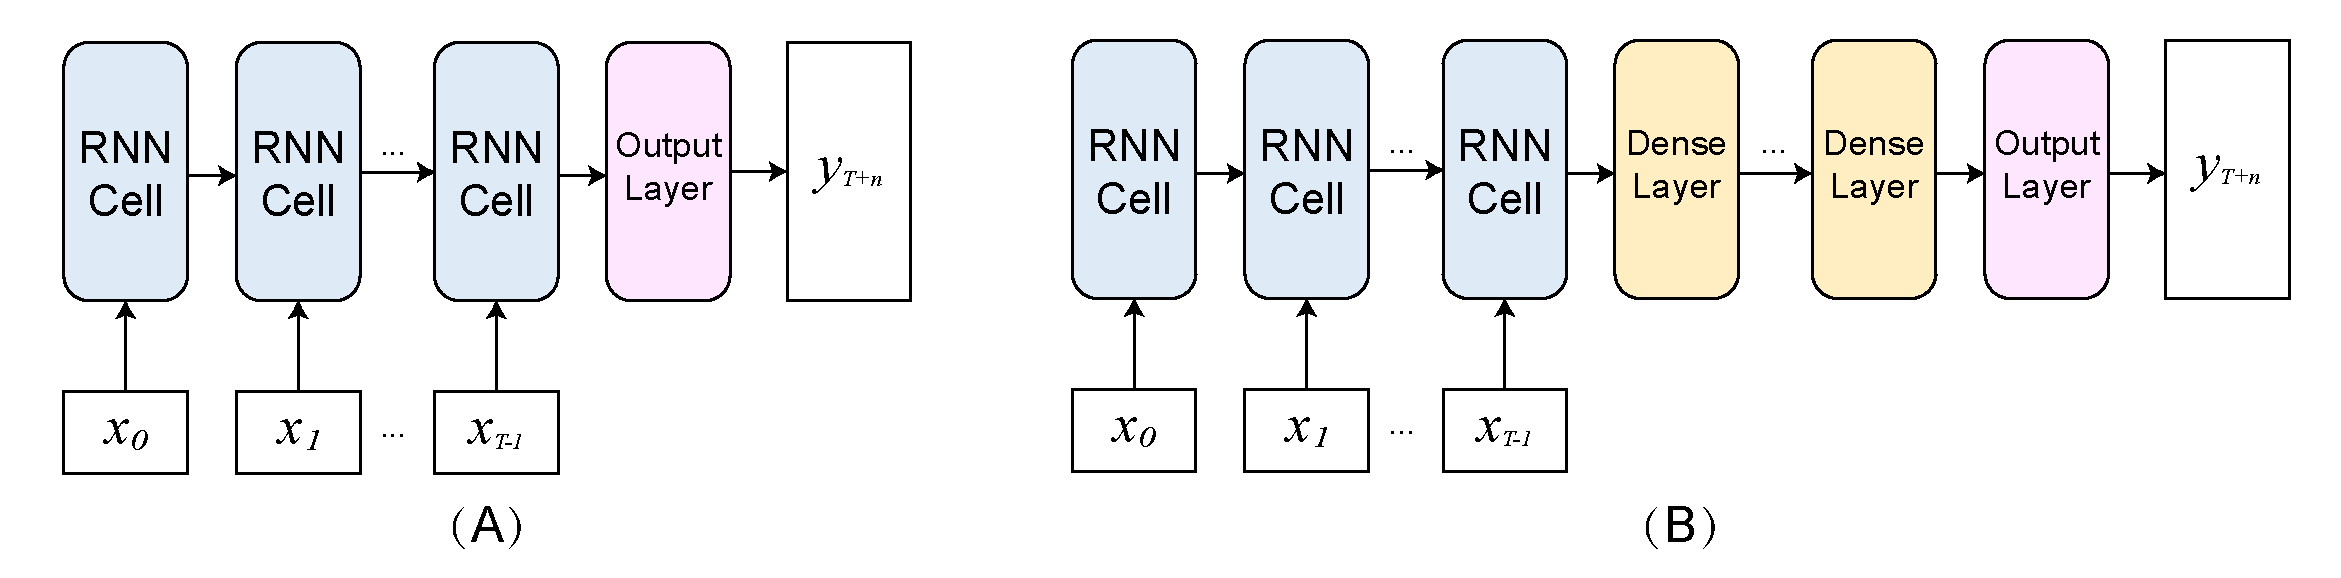
\includegraphics[width=0.9\textwidth]{figure/MultiRNNExplorer/model_description/model.pdf}
	\vspace{-5mm}
	\caption{\UC{RNN Architectures considered in our experiments: A) RNN: the RNN layer is directly connected to the output layer; B) RNN-Dense: adding dense layers between the RNN layer and the output layer.}
	}
	\label{fig:model_type}
\end{figure}

